\documentclass{article}

\usepackage{graphicx}
\usepackage{tikz}
\usepackage{tikzsymbols}
\usetikzlibrary{calc,patterns,shapes.geometric}
\pagestyle{empty}
\usepackage[margin=0pt]{geometry}
\geometry{papersize={14in,12in}}

\def\centerarc[#1](#2)(#3:#4:#5){\draw[#1] ($(#2)+({#5*cos(#3)},{#5*sin(#3)})$) arc (#3:#4:#5);}

\begin{document}
	\begin{figure}
		\centering
		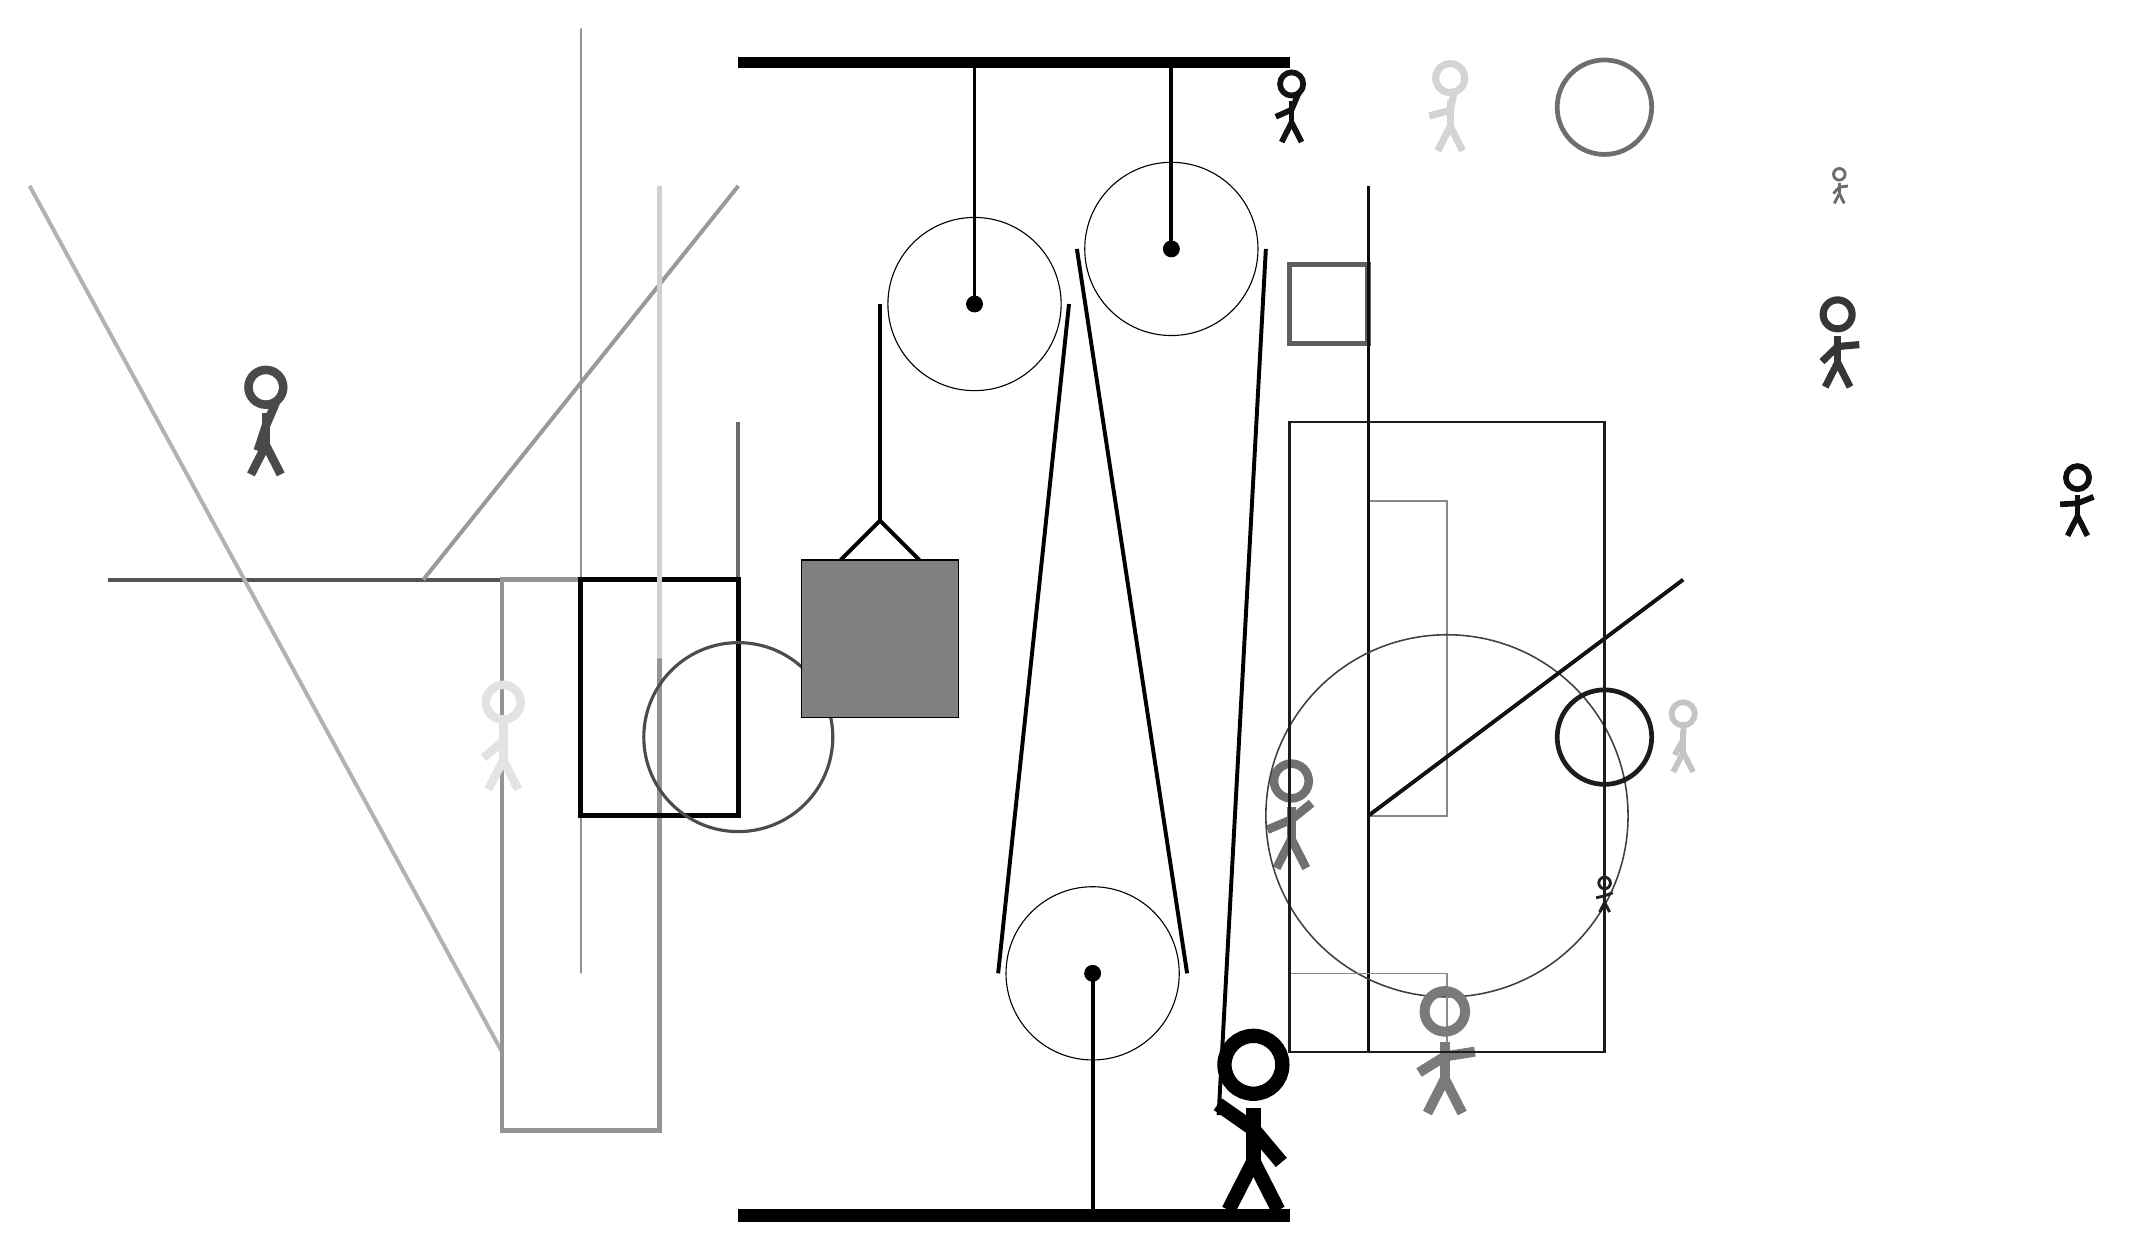
\begin{tikzpicture}
			%%%%% START %%%%%
			
			\draw[fill=black] (-2, 11.5) rectangle (5, 11.625);
			
			\draw (1, 8.5) circle (1.1);
			\draw[fill=black] (1, 8.5) circle (0.1);
			\draw[line width=0.5mm]  (1, 11.5) -- (1, 8.5);
			
			\draw[line width=0.5mm, color=black!58](-2, 7) -- (-2, 4);
			
			\draw[line width=0.2mm, color=black!43] (-4, 12) rectangle (-4, 0);
			\draw[line width=0.5mm, color=black!67](-2, 5) -- (-10, 5);
			\draw[line width=0.5mm, color=black!30](-5, -1) -- (-11, 10);
			\node[line width=0.7mm, color=black!56] at (5, 2) {\Strichmaxerl[6][23][39]};
			\node[line width=0.5mm, color=black!79] at (12, 8) {\Strichmaxerl[5][44][5]};
			\draw[line width=0.7mm, color=black!63] (5, 9) rectangle (6, 8);
			
			\draw[line width=0.5mm, color=black!40](-2, 10) -- (-6, 5);
			\node[line width=0.3mm, color=black!93] at (5, 11) {\Strichmaxerl[4][24][67]};
			\draw[line width=0.6mm, color=black!42] (-3, -2) rectangle (-5, 5);
			\draw[line width=0.3mm, color=black!47] (6, 2) rectangle (7, 6);
			\draw[line width=0.4mm, color=black!95] (6, -1) rectangle (6, 10);
			\node[line width=0.7mm, color=black!11] at (-5, 3) {\Strichmaxerl[6][41][90]};
			
			\node[line width=0.3mm, color=black!94] at (15, 6) {\Strichmaxerl[4][3][22]};
			\draw [line width=0.2mm, color=black!75](7, 2) circle (2.3);
			\node[line width=0.4mm, color=black!23] at (10, 3) {\Strichmaxerl[4][61][88]};
			
			\draw[line width=0.6mm, color=black!99] (-2, 2) rectangle (-4, 5);
			
			\draw[line width=0.5mm, color=black!93](10, 5) -- (6, 2);
			\node[line width=0.3mm, color=black!58] at (12, 10) {\Strichmaxerl[2][47][8]};
			
			\draw [line width=0.4mm, color=black!70](-2, 3) circle (1.2);
			\draw[line width=0.2mm, color=black!46] (7, 0) rectangle (5, -1);
			
			\node[line width=0.2mm, color=black!17] at (7, 11) {\Strichmaxerl[5][15][78]};
			\draw [line width=0.6mm, color=black!57](9, 11) circle (0.6);
			\node[line width=0.6mm, color=black!52] at (7, -1) {\Strichmaxerl[7][32][9]};
			\node[line width=0.6mm, color=black!71] at (-8, 7) {\Strichmaxerl[6][72][67]};
			
			\draw [line width=0.6mm, color=black!89](9, 3) circle (0.6);
			\draw[line width=0.3mm, color=black!89] (5, 7) rectangle (9, -1);
			\node[line width=0.6mm, color=black!87] at (9, 1) {\Strichmaxerl[2][13][21]};
			
			\draw[line width=0.6mm, color=black!18] (-3, 10) rectangle (-3, 4);
			
			\draw[fill=white](2.5, 0.0) circle (1.1);
			\draw[fill=black] (2.5, 0.0) circle (0.1);
			\draw[line width=0.5mm]  (2.5, -3) -- (2.5, 0.0);
			
			\draw[fill=white](3.5, 9.2) circle (1.1);
			\draw[fill=black] (3.5, 9.2) circle (0.1);
			\draw[line width=0.5mm] (3.5, 11.5) -- (3.5, 9.2);
			
			\draw[line width=0.5mm] (-0.7, 5.25) -- (-0.2, 5.75) -- (0.3, 5.25);
			\draw[fill=black!50] (-1.2, 5.25) rectangle (0.8, 3.25);
			
			\draw[line width=0.5mm] (-0.2, 8.5) -- (-0.2, 5.75);
			\centerarc[line width=0.5mm](1, 8.5)(0:180:1.2000000000000002);
			\draw[line width=0.5mm](2.2, 8.5) -- (1.3, 0.0);
			\centerarc[line width=0.5mm](2.5, 0.0)(180:360:1.2000000000000002);
			\draw[line width=0.5mm](3.7, 0.0) -- (2.3, 9.2);
			\centerarc[line width=0.5mm](3.5, 9.2)(0:180:1.2000000000000002);
			\draw[line width=0.5mm](4.7, 9.2) -- (4.1, -1.8);
			
			\node at (4.5, -1.9) {\Strichmaxerl[10][-35][-50]};
			
			\draw[fill=black] (-2, -3) rectangle (5, -3.15);
			
			%%%%% END %%%%%
		\end{tikzpicture}
	\end{figure}	
\end{document}